%-*- coding: UTF-8 -*-

\documentclass[UTF8]{ctexart}
\usepackage{graphicx}
\usepackage{float}
\usepackage{amsmath}
\usepackage{amssymb}
\usepackage{yhmath}
\usepackage{amsthm}
\usepackage{esint}
\usepackage{geometry}
\usepackage{bigints}
\geometry{a4paper,centering,scale=0.8}
\usepackage[format=hang,font=small,textfont=it]{caption}
\usepackage[nottoc]{tocbibind}
\usepackage{setspace}		%使用间距宏包
\usepackage{ctex}
\usepackage{fontspec}
\usepackage{color}
\usepackage{etoolbox}
\usepackage{enumitem}
\usepackage{extarrows}
\usepackage{tikz}
\usepackage{pgfplots}
\newcommand*{\circled}[1]{\lower.7ex\hbox{\tikz\draw (0pt, 0pt)%
    circle (.5em) node {\makebox[1em][c]{\small #1}};}}
\robustify{\circled}

%带圈数字配置,会改变字体,不用可注释
%\usepackage{libertine}
%% \libcirc and \libcircblk display their '0' if the parameter is out of range
%\newcommand{\libcirc}[1]{\pgfmathparse{
%    ifthenelse(#1 > 0 && #1 < 21, Hex(9311+#1), Hex(9450)
%    }\libertineGlyph{uni\pgfmathresult}}
%\newcommand{\libcircdbl}[1]{\pgfmathparse{Hex(9460+#1)}\libertineGlyph{uni\pgfmathresult}}
%\newcommand{\libcircblk}[1]{\pgfmathparse{
%    ifthenelse(#1 > 0 && #1 < 11, Hex(10101+#1),
%        ifthenelse(#1 > 10 && #1 < 21, Hex(9450-10+#1),
%            Hex(9471)
%        )
%    )
%    }\libertineGlyph{uni\pgfmathresult}}
%
%\newcommand{\juncirc}[1]{{\fontspec[Ligatures=Discretionary]{Junicode}[#1]}}
%\newcommand{\juncircdbl}[1]{{\fontspec[Ligatures=Discretionary]{Junicode}[[#1]]}}
%\newcommand{\juncircblk}[1]{{\fontspec[Ligatures=Discretionary]{Junicode}<#1>}}

\pgfplotsset{compat=newest}% use newest version

%begin画星形线
\newcommand*{\A}{2}
\newcommand*{\num}{2.2}

 % X 的参数方程
\pgfmathdeclarefunction{SolutionX}{1}{%
    \pgfmathparse{\A*(cos(deg(\t)))^3}%
}

 % Y 的参数方程
\pgfmathdeclarefunction{SolutionY}{1}{%
    \pgfmathparse{\A*(sin(deg(\t)))^3}%
}

 % define elegant style
\tikzset{elegant/.style={smooth, red, thick, samples=101}}

%end画星形线

%%使section后面也有引导点,暂时无此需要
\usepackage{titletoc} 
%\titlecontents{section}[0pt]{\addvspace{2pt}\filright}
%{\contentspush{\thecontentslabel\ }}
%{}{\titlerule*[8pt]{.}\contentspage}

%新命令
\newcommand\dif{\mathrm{d}}
\newcommand\no{\noindent}
\newcommand\dis{\displaystyle}
\newcommand\ls{\leqslant}
\newcommand\gs{\geqslant}

\newcommand\limit{\dis\lim\limits}
\newcommand\limn{\dis\lim\limits_{n\to\infty}}
\newcommand\limxz{\dis\lim\limits_{x\to0}}
\newcommand\limxi{\dis\lim\limits_{x\to\infty}}
\newcommand\limxpi{\dis\lim\limits_{x\to+\infty}}
\newcommand\limxni{\dis\lim\limits_{x\to-\infty}}

\newcommand\sumn{\dis\sum\limits_{n=1}^{\infty}}
\newcommand\sumnz{\dis\sum\limits_{n=0}^{\infty}}
\newcommand\sumk{\dis\sum\limits_{k=1}^{\infty}}
\newcommand\sumkz{\dis\sum\limits_{k=0}^{\infty}}
\newcommand\sumin{\dis\sum\limits_{i=1}^{n}}
\newcommand\sumizn{\dis\sum\limits_{i=0}^{n}}
\newcommand\sumkn{\dis\sum\limits_{k=0}^n}
\newcommand\sumkfn{\dis\sum\limits_{k=1}^n}

\newcommand\pzx{\dis\frac{\partial z}{\partial x}}
\newcommand\pzy{\dis\frac{\partial z}{\partial y}}

\newcommand\pfx{\dis\frac{\partial f}{\partial x}}
\newcommand\pfy{\dis\frac{\partial f}{\partial x}}

\newcommand\pzxx{\dis\frac{\partial^2 z}{\partial x^2}}
\newcommand\pzxy{\dis\frac{\partial^2 z}{\partial x\partial y}}
\newcommand\pzyx{\dis\frac{\partial^2 z}{\partial y\partial x}}
\newcommand\pzyy{\dis\frac{\partial^2 z}{\partial y^2}}

\newcommand\pfxx{\dis\frac{\partial^2 f}{\partial x^2}}
\newcommand\pfxy{\dis\frac{\partial^2 f}{\partial x\partial y}}
\newcommand\pfyx{\dis\frac{\partial^2 f}{\partial y\partial x}}
\newcommand\pfyy{\dis\frac{\partial^2 f}{\partial y^2}}

\newcommand\intzi{\dis\int_{0}^{+\infty}}
\newcommand\intd{\dis\int}
\newcommand\intab{\dis\int_a^b}

%调整分数数字与分数线的间距
%\renewcommand{\dfrac}[2]{{
%\renewcommand{\arraystretch}{1.375}
%\begingroup\displaystyle
%\rule[0pt]{0pt}{11pt}#1\endgroup%
%\over\displaystyle\rule[-3pt]{0pt}{11pt}#2
%}}%

\newenvironment{mfrac}[2]%
{\raise0.5ex\hbox{$#1$}\! \left/ \! \lower0.5ex\hbox{$#2$}\right.}

%定义新数学符号
\DeclareMathOperator{\sgn}{sgn}
\DeclareMathOperator{\arccot}{arccot}

\title{\heiti 全国大学生数学竞赛习题总结}
\author{\kaishu 唐渊 (XuanYuan\_huan)}
\date{\today}

\bibliographystyle{plain}

%开始写文章
\begin{document}
    
\maketitle

\newpage

\tableofcontents

\newpage

\section{一元函数的极限与连续}

\subsection{极限}

\begin{spacing}{2}

\no 1. 极限性质

局部有界性,局部保号性,单调有界原理,夹逼准则

\no 2.等价无穷小:乘除、幂指型替换

$\sin x \sim x-\dfrac{1}{6}x^3 \qquad \arcsin x \sim x+\dfrac{1}{6}x^3\
\qquad \cos x \sim 1-\dfrac{1}{2}x^2+\dfrac{1}{24}x^4 \qquad 
\arccos x \sim \dfrac{\pi}{2}-x-\dfrac{1}{6}x^3  $

\vspace{0.3cm}

$ \tan x \sim x+\dfrac{1}{3}x^3\qquad \arctan x \sim x-\dfrac{1}{3}x^3 \qquad
e^x\sim 1+x+\dfrac{1}{2}x^2+\dfrac{1}{6}x^3\qquad \ln(1+x)\sim x-\dfrac{1}{2}x^2
+\dfrac{1}{3}x^3$

\vspace{0.3cm}

$(1+x)^\lambda-1\sim \lambda x+\dfrac{\lambda(\lambda-1)}{2}x^2,\ \lambda\neq0
\qquad (1+x)^{\tfrac{1}{x}}\sim e\left(1-\dfrac{1}{2}x+\dfrac{11}{24}x^2\right)$

\no 3. L'Hospital法则

适用于$\dfrac{0}{0},\ \dfrac{\infty}{\infty},\ \dfrac{*}{\infty}\left(\text{推广型}\dfrac{\infty}{\infty}\right)$,以下各种形式可以转化:

\begin{enumerate}[itemindent=1.4em, label=(\arabic*)]

\item $0\cdot\infty\longrightarrow\mfrac{0}{\dfrac{1}{\infty}}$ or $\mfrac{\infty}{\dfrac{1}{0}}$

\item $\infty\pm\infty'\longrightarrow\mfrac{\left(\dfrac{1}{\infty'}\pm\dfrac{1}{\infty}\right)}{\dfrac{1}{\infty\cdot\infty'}}$

\item $1^\infty,\ 0^0,\ \infty^0\longrightarrow$幂指转化

\end{enumerate}

\no4.极限变量代换:归结原则(Heine定理)

$\limit_{x\to a}f(x)=A\Leftrightarrow\forall\left\{x_n\right\}\to a,\limn f(x_n)=A.$

函数极限$\leftrightarrow$数列极限

\no5.子数列

$\limn x_n=A\Leftrightarrow \forall \left\{x_{k_n}\right\}\subseteq\{x_n\},\ \limn x_{k_n}=A.$

子数列若互不相交,则分别取极限,值相同即可.

\no6. Stolz定理:数列极限的洛必达法则$\left(\mfrac{*}{\infty}\right)$

$\{b_n\}\nearrow\infty\ \Longrightarrow\ \limn\dfrac{a_n}{b_n}=\limn\dfrac{a_n-a_{n-1}}{b_n-b_{n-1}}.$

\no7.常用极限

$a>0,\  \limit_{x\to0^+}x^a\ln x=0.$

\no8.习题总结

\begin{enumerate}[itemindent=1.4em, label=(\arabic*)]

\item 等价无穷小的派生

\item 极限的平均值定理$\Longleftarrow$ Stolz定理

\item 迭代数列的极限

\begin{enumerate}[itemindent=1.4em, label=(\alph*)]

\item 单调有界原理:数学归纳法

\item 夹逼:假设极限存在,再证明其存在。无限递推$+$等比数列$+$微分中值定理

\end{enumerate}

\item 比值法与根值法求极限

\setlength\parindent{2em}$\limn \left|\dfrac{a_n}{a_{n-1}}\right|=q,\ 
\limn\sqrt[\leftroot{-3}\uproot{+7}n]{|a_n|}=q.$

\item $n\to\infty,\ n^{p+1}-(n-1)^{p+1}\sim n^p\cdot (p+1).$

\item Stolz定理:一般用于$\lim\dfrac{\sum f(n)}{n^\alpha},\ \alpha\in\mathbb{R}$.

\item 相乘相消缺项,根号下平方放缩。

\item 三项递推,考虑两项组合;累加求和,考虑级数求和。

\item 连乘积:连续平方差,连续倍角公式。

\item 迭代数列求出极限反证时,幂函数直接做,其他函数可用Lagrange中值定理或直接Taylor.

\item 已知数列极限$\limn x_n=a$,常可反设数列$x_n=a+\alpha_n$,其中$\alpha_n\to0\ (n\to\infty).$

\item 函数极限:

\begin{enumerate}[itemindent=1.4em, label=(\alph*)]

\item 一般不定式$\longrightarrow$ Taylor.

\item 幂指型$(1^\infty)\ \alpha^\beta\longrightarrow e^{\beta(\alpha-1)}.$

\item 根式相减$\longrightarrow$分子有理化

\item 组合趋零$\longrightarrow$提化单趋零

\item 同函数相减$\longrightarrow$ Lagrange中值定理

\end{enumerate}

\end{enumerate}

\subsection{连续}

\no1.内容要点

\begin{enumerate}[itemindent=1.4em, label=(\arabic*)]

\item 定义:$\limit_{x\to x_0}f(x)=f(x_0).$

\item $\text{间断点:}\left\{
\begin{aligned}
&\text{第一类:} \left\{ \begin{aligned} \text{可去间断点}\\
\text{跳跃间断点}
\end{aligned}
\right. \\
&\text{第二类:}			%&可以设置对齐位置
\left\{ \begin{aligned} \text{无穷间断点}\\
\text{振荡间断点}
\end{aligned}
\right. 
\end{aligned}
\right.$

\item 闭区间连续函数:最值定理,介值定理,零点定理

\end{enumerate}

\no2.习题总结

\begin{enumerate}[itemindent=1.4em, label=(\arabic*)]

\item 由函数恒等式确定函数方程

$\left\{\begin{aligned}
\text{一元:}&\text{降无限迭代,极限聚已知}\\
\text{二元:}&\text{正有理数}\Rightarrow\text{负有理数}\Rightarrow
\text{无理数(有理数的稠密性)}\\
&\left(\dfrac{1}{n}\to\dfrac{m}{n}\right)\Rightarrow
(x\to -x)\Rightarrow\left(\limn r_n\right)\\
&\text{前提:}f(x)\text{显隐函数的连续性}
\end{aligned}\right.$

\item 存在性等式

$\left\{\begin{aligned}
&\text{反证法:差值构造,不妨恒大于零,推出矛盾!}\\
&\text{差值构造,零点定理}\\
&\text{最值定理+介值定理}
\end{aligned}\right.$

\item 证明连续性

$\left\{\begin{aligned}
&\text{定义:}\limit_{\Delta x\to0}\big[f(x+\Delta x)-f(x)\big]=0\\
&\text{双边极限,注意夹逼}\\
&\text{函数间初等运算、复合运算,保连续性}
\end{aligned}\right.$

\end{enumerate}

\newpage

\section{一元函数微分学}

\subsection{导数与微分}

\no1.微分符号的飘逸性

\no2.高阶导数

$\begin{aligned}
&(uv)^{(n)}=\sumkn C_{n}^k\cdot u^{(k)}v^{(n-k)},\  C_{n}^k=\binom{n}{k}.\\
&(a^x)^{(n)}=a^x\ln^n a,\qquad\qquad\qquad\qquad\quad (\log_a x)^{(n)}=(-1)^{n-1}
\dfrac{(n-1)!}{x^n\ln a}.\\
&(\cos x)^{(n)}=\cos\left(x+n\cdot\dfrac{\pi}{2}\right),\qquad\qquad
(\sin x)^{(n)}=\sin\left(x+n\cdot\dfrac{\pi}{2}\right).\\
&\left(\dfrac{1}{x+a}\right)^{(n)}=(-1)^n\dfrac{n!}{(x+a)^{n+1}}, \qquad
\left(\dfrac{1}{a-x}\right)^{(n)}=\dfrac{n!}{(a-x)^{n+1}}.\\
\end{aligned}$

\vspace{0.5cm}

\no3.习题总结

\begin{enumerate}[itemindent=1.4em, label=(\arabic*)]

\item 求一点导数,有时导数定义更简捷:$f'(x_0)=\limit_{x\to x_0}\dfrac{f(x)-f(x_0)}{x-x_0}.$

\item $n\ \text{阶导数:}\left\{\begin{aligned}
&\text{公式法}\\
&\text{Leibniz求递推公式,保持方程为一次}\\
\end{aligned}\right.$

\item 幂指型求导$\longrightarrow$对数求导法

\item 导函数的极限定理:$\exists\limit_{x\to x_0}f'(x),\ \limit_{x\to x_0}f(x)=f(x_0)
\Longrightarrow\exists f'(x_0)=\limit_{x\to x_0}f'(x_0).$

$\text{注意:}\left\{\begin{aligned}
&\limit_{x\to x_0}\longleftrightarrow\limit_{x\to x_0^+}
\longleftrightarrow\limit_{x\to x_0^-}\text{可以替换}\\
&\limit_{x\to x_0}f'(x_0)\text{不存在}\nRightarrow f'(x_0)\text{不存在}\\
\end{aligned}\right.$

\item 导函数的介值定理(Darboux定理)

$f(x)$在$[a,b]$上可导,且$f'(a)\neq f'(b)$,则$\forall\ r\in 
\big[\min\{f'(a),f'(b)\},\max\{f'(a),f'(b)\}\big],$

$\exists\ \bar{x}\in(a,b),\ s.t.\ r=f'(\bar{x}).$

\item 由参数方程求高阶导数:$x=x(t),\ y=y(t),\ y'_x=\dfrac{y'_t}{x'_t},\ 
y''_{xx}=\dfrac{(y'_x)'_t}{x'_t},\ \cdots,\ y_x^{(n)}=\dfrac{\left(y_{x}^{(n-1)}\right)'_t}{x'_t}.$

\item 积化和差:组二减一,减三和,再四分

$\sin\alpha\sin\beta\sin\gamma=\dfrac{1}{4}\big[\sin(\alpha+\beta-\gamma)
+\sin(\alpha+\gamma-\beta)+\sin(\beta+\gamma-\alpha)
-\sin(\alpha+\beta+\gamma)\big].$

\end{enumerate}

\subsection{微分中值定理}

\no1.中值定理:闭区间连续,开区间可导

\vspace{0.4cm}

$\left\{\begin{aligned}
&f(a)=f(b),\Rightarrow\exists\ \xi\in(a,b),\ f'(\xi)=0;\\
&\Rightarrow\exists\ \xi\in(a,b),\ f(b)-f(a)=f'(\xi)(b-a);\\
&g'(x)\neq0,\ \Rightarrow\exists\ \xi\in(a,b),\ \dfrac{f'(\xi)}{g'(\xi)}=\dfrac{f(b)-f(a)}{g(b)-g(a)}.
\end{aligned}\right.$

\vspace{0.4cm}

\no2.凹凸性

凹函数$f(x)\Leftrightarrow f(q_1x_1+q_2x_2)\ls q_1f(x_1)+q_2f(x_2),\ q_1+q_2=1,
\ q_1,\ q_2>0.$

\vspace{0.3cm}

$\Leftrightarrow f\left(\sumkfn q_kx_k\right)\ls\sumkfn q_kf(x_k),
\ \sumkfn q_k=1,\ q_k>0,\ k=1,2,\cdots,n.$

\vspace{0.3cm}

$\Leftrightarrow f'(x)\nearrow\ \Leftrightarrow f''(x)\gs0.$

凸函数则以上各式不等号方向相反。

\no3.极值与最值

\begin{enumerate}[itemindent=1.4em, label=(\arabic*)]

\item $f(x)$在$\overset{o}{U} (x_0)$上有定义,$\forall \ x\in \overset{o}{U}(x_0),
\ f(x)<f(x_0)$,则$f(x_0)$为极大值。

\item (Fermat引理) 若极值$x_0$处可导,则$f'(x_0)=0.$

\item $\text{判别:}\left\{\begin{aligned}
&\text{左右邻域导数符号正负判别}\\
&\text{二阶导数判别}\\
\end{aligned}\right.$

\item 唯一极值,极值即最值。

\end{enumerate}

\no4.习题总结

\begin{enumerate}[itemindent=1.4em, label=(\arabic*)]

\item $\left\{\begin{aligned}
&\text{单中值问题:微分方程法,} F(x,y)=C.\\
&\text{多中值问题:Lagrange中值定理+连续介值定理;分母相加分区间,分子相加分函值。}
\end{aligned}\right.$

\item Taylor展开:代入法,运算法,复合法;注意合并同类项,勿丢项。

\item 无穷区间Rolle定理:通过复合函数将$\infty$化为具体值。

\item 高阶导数相关不等式问题:

高阶导则泰勒展,单点定则整体动。定点必为高导点,和限小则独限大。

无穷区间任意展,闭区展开代端点。若是端点值相等,定点区间可半分。

\item 凹凸性与不等式:相乘不通转相除,幂指开对数。

\item $\text{极值与最值:}\left\{\begin{aligned}
&\text{极值点:奇阶为零偶非零,偶重零极奇不极。}\\
&\text{画草图:奇穿偶不穿。}\\
\end{aligned}\right.$
\end{enumerate}

\newpage

\section{不定积分与定积分}

\subsection{不定积分}

\no1.基本积分表

\begin{spacing}{3}
$\intd\dfrac{1}{x^2+a^2}\dif x=\dfrac{1}{a}\arctan \dfrac{x}{a}+C.
\qquad\qquad
\intd\dfrac{1}{x^2-a^2}\dif x=\dfrac{1}{2a}\ln\left| \dfrac{x-a}{x+a}\right|+C$.

$\intd\dfrac{1}{(x^2+a^2)^2}\dif x=\dfrac{1}{2a^3}\left(\arctan \dfrac{x}{a}
+\dfrac{ax}{x^2+a^2}\right)+C$.

$\intd\dfrac{1}{\sqrt{x^2\pm a^2}}\dif x=\ln \left|x+\sqrt{x^2\pm a^2}\right|+C.
\qquad\qquad
\intd\dfrac{1}{\sqrt{a^2- x^2}}\dif x=\arcsin \dfrac{x}{a}+C$.

$\intd\sqrt{a^2-x^2}\dif x=\frac{1}{2}\left(x\sqrt{a^2-x^2}+a^2
\arcsin\frac{x}{a}\right)+C$.

$\intd\sqrt{x^2\pm a^2}\dif x=\frac{1}{2}\left(x\sqrt{x^2\pm a^2}\pm a^2
\ln\left|x+\sqrt{x^2\pm a^2}\right| \right)+C$.

$\begin{aligned}
\intd\frac{1}{x^4+1}\dif x&=\frac{1}{2}\intd\frac{x^2+1}{x^4+1}\dif x-
\frac{1}{2}\intd\frac{x^2-1}{x^4+1}\dif x
=\frac{1}{2}\dis\bigintsss\frac{1+\dfrac{1}{x^2}}{x^2+\dfrac{1}{x^2}}\dif x
-\frac{1}{2}\bigintsss\frac{1-\dfrac{1}{x^2}}{x^2+\dfrac{1}{x^2}}\dif x \\
&=\frac{1}{2}\bigintsss\frac{\dif \left(x-\dfrac{1}{x}\right)}{\left(x-\dfrac{1}{x}\right)^2+2}
-\frac{1}{2}\bigintsss\frac{\dif \left(x+\dfrac{1}{x}\right)}{\left(x+\dfrac{1}{x}\right)^2-2}.
\end{aligned}$

\vspace{0.4cm}

$\intd\frac{\dif x}{\sqrt[^n\!]{1+x^n}}\xlongequal{x=\tfrac{1}{t}}
-\intd\frac{\dif t^n}{nt^n\sqrt[^n\!]{t^n+1}}\xlongequal{u=t^n}
-\intd\frac{\dif u}{nu\sqrt[^n\!]{u+1}}\xlongequal{v=\sqrt[^n\!]{u+1}}
-\intd\frac{v^{n-2}}{v^n-1}\dif v.$

(分母同$x$次,先用倒代换)

$\intd\tan x\dif x=-\ln|\cos x|+C.
\qquad\qquad
\intd\cot x\dif x=\ln|\sin x|+C.$

$\intd\tan^2 x\dif x=\tan x-x+C.
\qquad\qquad
\intd\cot^2 x\dif x=-\cot x-x+C.$

$\intd \sec x\dif x=\ln|\sec x+\tan x|+C.
\qquad\qquad
\intd\csc x\dif x=\ln|\csc x-\cot x|+C.$

$\intd\frac{A\sin x+B\cos x}{C\sin x+D\cos x}\dif x
=m\cdot x+n\cdot \ln|C\sin x+D\cos x|+C',\ 
m=\frac{AC+BD}{C^2+D^2},\ n=\frac{BC-AD}{C^2+D^2}.$

\end{spacing}

\no2.积分方法

\begin{enumerate}[itemindent=1.4em, label=(\arabic*)]

\item 线性分解法

\item 凑微分法

\item 换元法

$\intd R(x,\sqrt{a^2-x^2})\dif x\longrightarrow x=a\sin t$

$\intd R(x,\sqrt{a^2+x^2})\dif x\longrightarrow x=a\tan t$

$\intd R(x,\sqrt{x^2-a^2})\dif x\longrightarrow x=a\sec t$

$\intd R(\sin x,\cos x)\dif x\longrightarrow 
\left\{\begin{aligned}
&t=\tan\frac{x}{2},\ 
\dif x=\frac{2}{1+t^2}\dif t,\ \sin x=\frac{2t}{1+t^2},\ 
\cos x=\frac{1-t^2}{1+t^2}\\
&R(\sin x,-\cos x)=-R(\sin x,\cos x)\longrightarrow t=\sin x\\
&R(-\sin x,\cos x)=-R(\sin x,\cos x)\longrightarrow t=\cos x\\
&R(-\sin x,-\cos x)=R(\sin x,\cos x)\longrightarrow t=\tan x\\
\end{aligned}\right.$

$\intd R\left(x,\sqrt[^n\!]{ax+b}\right)\dif x\longrightarrow u=\sqrt[^n\!]{ax+b}$

$\intd R\left(x,\sqrt[\leftroot{-3}\uproot{+16}n]
{\dfrac{ax+b}{cx+d}}\right)\dif x\longrightarrow 
u=\sqrt[\leftroot{-3}\uproot{+16}n]{\dfrac{ax+b}{cx+d}}$

$\intd R(\sqrt[^p\!]{x},\sqrt[^q\!]{x})\dif x\longrightarrow u=\sqrt[^n\!]{x},\ $
$n$为$p,\ q$的最小公倍数

$\intd\frac{P_m(x)}{Q_n(x)}\dif x\longrightarrow t=\frac{1}{x},\ m<<n.$
(倒代换,分$x>0$和$x<0$讨论,$x<0$的情况可同理)

\item 分部积分法:反对幂指三(前$u$后$v$),$\intd u\dif v=uv-\intd v\dif u$

\end{enumerate}

\no3.有理函数积分

长除法$\longrightarrow$真分式分解$\longrightarrow$待定系数法$\longrightarrow$
代入分母因式分解后的根,实根直接出系数,复根比较实部与虚部得出系数

\no4.原函数的封闭性

$P_n(x)\cdot e^{\lambda x}\xlongrightarrow{x=\ln t}P_n(\ln t)\cdot t^\lambda,\ 
\qquad
P_n(x)e^{ax}\cos bx+Q_n(x)e^{ax}\sin bx$

\no5.习题总结

\begin{enumerate}[itemindent=1.4em, label=(\arabic*)]

\item $\sumkn \cos (\alpha +k\beta)=\dfrac{\cos\left(\alpha+\dfrac{n}{2}\beta\right)
\sin \dfrac{n+1}{2}\beta}{\sin\dfrac{\beta}{2}},
\qquad
\sumkn \sin (\alpha +k\beta)=\dfrac{\sin\left(\alpha+\dfrac{n}{2}\beta\right)
\sin \dfrac{n+1}{2}\beta}{\sin\dfrac{\beta}{2}}$

\item 分部积分:建立方程,构造递推公式

\item 三角换元可借助画三角形寻找相关函数表达式:
$\sim$表示相差常数$\left(\dfrac{\pi}{2}\right)$或相等

$\begin{aligned}
&\arcsin x\sim-\arccos x\sim\arctan\dfrac{x}{\sqrt{1-x^2}},\qquad
-\arcsin x\sim\arccos x\sim\arctan\dfrac{\sqrt{1-x^2}}{x}\\
&\arcsin \dfrac{1}{x}\sim-\arccos \dfrac{1}{x}\sim\arctan\dfrac{1}{\sqrt{1-x^2}},\qquad
-\arcsin \dfrac{1}{x}\sim\arccos \dfrac{1}{x}\sim\arctan\sqrt{1-x^2}\\
\end{aligned}$

\item $\intd\cos^mx\sin^nx\dif x$:双正偶数用倍角,其他情形用换元

\end{enumerate}

\subsection{定积分}

\no1.定积分性质

\begin{enumerate}[itemindent=1.4em, label=(\arabic*)]

\item 积分单调性

$\forall x\in[a,b],\ f(x)\ls g(x)\Longrightarrow\intab f(x)\dif x\ls\intab g(x)\dif x\Longrightarrow\left|\intab f(x)\dif x\right|\ls\intab|f(x)|\dif x.$

\item 积分保号性

\item 积分恒等性(证明常用)

$f(x),\ g(x)$连续,$\ \forall x\in[a,b],\ f(x)\ls g(x),\ \intab f(x)\dif x=\intab g(x)\dif  x
\Longrightarrow f(x)\equiv g(x).$

\item 积分估值公式

\item 积分中值定理

\begin{enumerate}[itemindent=1.4em, label=(\alph*)]

\item 积分第一中值定理

$f(x)$连续,$\ g(x)$不变号, $\exists\ \xi\in[a,b],\ s.t.\ \intab f(x)g(x)\dif x
=f(\xi)\intab g(x)\dif x.$

Let $g(x)=1\Longrightarrow \intab f(x)\dif x=f(\xi)(b-a).$

\item \textcolor[rgb]{1,0,0}{积分第二中值定理}

(i) $f(x),\ g(x)$在闭区间$[a,b]$上可积,且$f(x)$为单调函数
$\Longrightarrow\exists\ \xi\in[a,b],\ s.t.\ $

\centerline{$\intab f(x)g(x)\dif x=f(a)\intd_a^\xi g(x)\dif x+f(b)\intd_\xi^bg(x)\dif x.$}

Let $g(x)=1\Longrightarrow\intab f(x)\dif x=f(a)(\xi-a)+f(b)(b-\xi).$

(ii) $f(x),\ g(x)$在闭区间$[a,b]$上可积,$f(x)\gs0$为单调递减函数
$\Longrightarrow\exists\ \xi\in[a,b],\ s.t.\ $

\centerline{$\intab f(x)g(x)\dif x=f(a)\intd_a^\xi g(x)\dif x.$}

Let $g(x)=1\Longrightarrow\intab f(x)\dif x=f(a)(\xi-a).$

(iii) $f(x),\ g(x)$在闭区间$[a,b]$上可积,$f(x)\gs0$为单调递增函数
$\Longrightarrow\exists\ \xi\in[a,b],\ s.t.\ $

\centerline{$\intab f(x)g(x)\dif x=f(b)\intd_\xi^bg(x)\dif x.$}

Let $g(x)=1\Longrightarrow\intab f(x)\dif x=f(b)(b-\xi).$

\end{enumerate}

\end{enumerate}

\no2.变限积分

含限变限,换元或提出含限$f(x)$;双变量,考虑对另一变量求导

\no3.定积分简算

\begin{enumerate}[itemindent=1.4em, label=(\arabic*)]

\item 对称奇偶性

\item 周期性

\item \textcolor[rgb]{1,0,0}{点火公式},到乘单1或$\dfrac{\pi}{2}$止

$I_n=\intd_0^{\tfrac{\pi}{2}}\sin^nx\dif x
=\intd_0^{\tfrac{\pi}{2}}\cos^nx\dif x
=\intd_0^{\tfrac{\pi}{2}}\sin^nkx\dif x
=\intd_0^{\tfrac{\pi}{2}}\cos^nkx\dif x$

\item 正余弦换元技巧:\textbf{区间再现}

$\intd_0^{\pi}xf(\sin x)\dif x=\dfrac{\pi}{2}\intd_0^\pi f(\sin x)\dif x,\ x=\pi-t.
\qquad\intd_0^{\pi}xf(\cos x)\dif x$不具有这个性质.

\vspace{0.3cm}

$\intd_0^\pi \dfrac{\sin^{2n}x}{\sin^{2n}x+\cos^{2n}x}\dif x=
\intd_0^\pi \dfrac{\cos^{2n}x}{\sin^{2n}x+\cos^{2n}x}\dif x=\dfrac{\pi}{2},\ 
x=\dfrac{\pi}{2}-t.$

\vspace{0.3cm}

$\begin{aligned}
\intd_0^{\tfrac{\pi}{2}}\ln (\sin x)\dif x&=\intd_0^{\tfrac{\pi}{2}}\ln (\cos x)\dif x=
\dfrac{1}{2}\intd_0^{\tfrac{\pi}{2}}\ln \left(\dfrac{1}{2}\sin 2x\right)\dif x\\
&=-\dfrac{\pi}{4}\ln 2+\dfrac{1}{2}\intd_0^{\tfrac{\pi}{2}}\ln (\sin x)\dif x=
-\dfrac{\pi}{2}\ln 2,\ x=\dfrac{\pi}{2}-t.\\
\end{aligned}$

$\begin{aligned}
\intd_0^{\tfrac{\pi}{4}}\ln(1+\tan x)\dif x
&=\intd_0^{\tfrac{\pi}{4}}\ln\left[1+\tan \left(\dfrac{\pi}{4}-x\right)\right]\dif x
=\intd_0^{\tfrac{\pi}{4}}\ln\left(1+\dfrac{1-\tan x}{1+\tan x}\right)\dif x\\
&=\intd_0^{\tfrac{\pi}{4}}\ln\dfrac{2}{1+\tan x}\dif x
=\dfrac{1}{2}\intd_0^{\tfrac{\pi}{4}}\ln2\ \dif x=\dfrac{\pi}{8}\ln2,\ x=\dfrac{\pi}{4}-t.\\
\end{aligned}$

\item 三角函数系的正交性

\item 含参积分:对参数求导

$\intd_0^{\tfrac{\pi}{2}}\ln\left(a^2\sin^2x+b^2\cos^2x\right)\dif x
\triangleq I(b)
=\intd_0^{b}I'(t)\dif t+I(0)
=\intd_0^{b}\dfrac{\pi}{|a|+t}\dif t+\pi\ln\dfrac{|a|}{2}
=\pi\ln\dfrac{|a|+|b|}{2}.$

$\intd_0^\pi\ln\left(1-2a\cos x+a^2\right)\dif x
\left\{\begin{aligned}
&\triangleq I(a)=\intd_0^{a}I'(t)\dif t+I(0)
=\dfrac{\pi}{2}-\dfrac{2}{a}\arctan\dfrac{1+a}{1-a}x\bigg|_0^{+\infty}=0,\ |a|<1\\
&=I(\pm1)=\intd_0^\pi\ln2(1\mp\cos x)\dif x=0,\qquad\qquad |a|=1\\
&\xlongequal{b=\tfrac{1}{a}}
\intd_0^\pi\ln\dfrac{b^2-2b\cos x+1}{b^2}\dif x
=I(b)-2\pi\ln|b|=2\pi\ln|a|,\ |a|>1\\
\end{aligned}\right.$

\textcolor[rgb]{1,0,0}{$\Longrightarrow\intd_0^\pi\ln(m\pm n\cos x)\dif x
=\intd_{-\tfrac{\pi}{2}}^{\tfrac{\pi}{2}}\ln(m\pm n\sin x)\dif x
=2\pi\ln\dfrac{\sqrt{m+n}+\sqrt{m-n}}{2},\ m\gs |n|\gs 0.$}

\end{enumerate}

\no4.广义积分:瑕积分与无穷积分

原函数取极限;无穷区间可以1分,取倒数合并

\no5.定积分在几何中的应用

\begin{enumerate}[itemindent=1.4em, label=(\arabic*)]

\item  微元法 ,一般参数方程的形式更好用

\item 弧长微元$\dis\dif s=\sqrt{(\dif x)^2+(\dif y)^2}=\sqrt{(x'_t)^2+(y'_t)^2}\dif t
=\sqrt{1+(y'_x)^2}\dif x=\sqrt{r^2+(r'_\theta)^2}\dif \theta.$

\item 空间直线方程可由直线在$xOy,\ yOz,\ zOx$其中任意两个面上的投影方程(两个面)限制

\item 最值问题:可以考虑分设两(多)个变量,外加两(多)变量之间关系式即可

\end{enumerate}

\no6.变项和(无穷和)的极限

\begin{enumerate}[itemindent=1.4em, label=(\arabic*)]

\item 定积分法

\item Lagrange型Taylor展开,例如$\sin x=x-\dfrac{\sin\xi}{2!}x^2,\ \xi\in(0,x).$

\item 夹逼极限$\longleftarrow$凑形式

\item $\limn\sum\limits_{j=\inf(n)}^{\sup(n)}f\left(\dfrac{j}{n}\right)\dfrac{1}{n}=
\bigintssss_{\lim\limits_{n\to\infty}\tfrac{\inf(n)}{n}}
^{\lim\limits_{n\to\infty}\tfrac{\sup(n)}{n}}f(x)\dif x.$

\item $A_n=\intab f(x)\dif x-\dfrac{b-a}{n}\dis\sum\limits_{k=1}^nf\left[
a+\dfrac{(b-a)k}{n}\right]\Longrightarrow\limn n\cdot A_n=\dfrac{b-a}{2}
\big[f(b)-f(a)\big].$

注:积分化和式,Lagrange中值定理可证。

\item $B_n=\intab f(x)\dif x-\dfrac{b-a}{n}\dis\sum\limits_{i=1}^nf\left[
a+(2i-1)\dfrac{b-a}{2n}\right]\Longrightarrow\limn n^2\cdot B_n=\dfrac{(b-a)^2}{24}\big[f'(b)-f'(a)\big].$

注:积分化和式,Taylor展开到第二项可证。

\item 定积分定义和式类Taylor展开

$\dfrac{b-a}{n}\dis\sum\limits_{k=1}^nf\left[a+\dfrac{(b-a)k}{n}\right]=
\intab f(x)\dif x+\sumk\dfrac{(-1)^k(b-a)^kB_k}{k!n^k}
\left[f^{(k-1)}(b)-f^{(k-1)}(a)\right]$, 

where $B_k$ is Bernoulli number, $B_0=1,\ B_1=-\dfrac{1}{2},\ B_2=\dfrac{1}{6},\cdots.$

注:积分化和式,借助Lagrange中值定理可得第一项,第二项则需要两次分部积分。

\end{enumerate}

\newpage

\section{多元函数微分学}

\subsection{函数与图形}

\no1.平面方程

$\dis\Sigma:A(x-x_0)+B(y-y_0)+C(z-z_0)=0,$ 法向量$\stackrel{\rightarrow}{n}=
(A,B,C),$

方向余弦$\dis\cos\alpha=\dfrac{A}{\sqrt{A^2+B^2+C^2}},\ 
\cos\beta=\dfrac{B}{\sqrt{A^2+B^2+C^2}},\ 
\cos\gamma=\dfrac{C}{\sqrt{A^2+B^2+C^2}},$ 

其中$\alpha=\left<\stackrel{\rightarrow}{n},\stackrel{\rightarrow}{i}\right>
=\left<\Sigma,yOz\right>,\ 
\beta=\left<\stackrel{\rightarrow}{n},\stackrel{\rightarrow}{j}\right>
=\left<\Sigma,zOx\right>,\ 
\gamma=\left<\stackrel{\rightarrow}{n},\stackrel{\rightarrow}{k}\right>
=\left<\Sigma,xOy\right>.$

\no2.直线方程

(1) 两面交线

(2) $\dfrac{x-x_0}{l}=\dfrac{y-y_0}{m}=\dfrac{z-z_0}{n};\ x=x_0+lt,\ 
y=y_0+mt,\ z=z_0+nt.$

\no3.二次曲面

单叶双曲面:$\dfrac{x^2}{a^2}+\dfrac{y^2}{b^2}-\dfrac{z^2}{c^2}=1,$
 双叶双曲面:$\dfrac{z^2}{c^2}-\dfrac{x^2}{a^2}-\dfrac{y^2}{b^2}=1.$
(单双看负号个数)

\no4.圆锥面铺平

$\dis z=a\sqrt{x^2+y^2},\ a=\cot \alpha,\ \alpha$为半顶角, 铺平后的圆心角
$\beta=2\pi\sin\alpha.$

\no5.旋转曲面的参数方程

$L:x=x(t),y=y(t),z=z(t),a\ls t\ls b,$ 绕$z$轴形成的曲面为

$\dis\Sigma: x=\sqrt{x^2(t)+y^2(t)}\cos\theta,\ 
y=\sqrt{x^2(t)+y^2(t)}\sin\theta,\ z=z(t),\ a\ls t\ls b,\ 0\ls\theta\ls 2\pi.$

\no6.直纹面上过一点的直线方程

参数方程代入法;因式分解比例法

\no7.顶点在原点的锥面:$n$次齐次方程$F(x,y,z)=0,\ $
其中$F(tx,ty,tz)=t^nF(x,y,z).$

\no8.投影方程:$xOy$面$\Longrightarrow$关于$z$的方程有解,得出$x,y$的限制方程.

\no9.空间特殊曲线:曲线定义;投影回溯(借助方向余弦).

\subsection{极限,连续与微分}

\no1.二重极限定义:$\limit_{(x,y)\to(x_0,y_0)}f(x,y)=A,\ $  
 连续:$\limit_{(x,y)\to(x_0,y_0)}f(x,y)=f(x_0,y_0).$

\begin{spacing}{2.5}

\no 偏导数:$z=f(x,y)\longrightarrow\pzx,\ \pfx,\ z'_x,\ z_x,\ f'_x,\ f_x,\ f'_1,\ f_1.$

\end{spacing}

\no 混合二阶偏导(注意次序):$\dfrac{\partial}{\partial y}\left(\pzx\right)=\pzxy,
\ f_{12},\ f''_{xy};
\qquad\dfrac{\partial}{\partial x}\left(\pzy\right)=\pzyx,\ f_{21},\ f''_{yx}.$

\no2.链式法则

\no 全微分:$\dis\Delta z=f(x+\Delta x,y+\Delta y)-f(x,y)=A\Delta x+B\Delta y+o(\rho),\ 
\rho=\sqrt{\Delta x^2+\Delta y^2}\Rightarrow\Delta z\triangleq\dif z.$

\no 全微分形式不变性

\no 隐函数求导法:直接求导法,公式法(全微分推出),全微分法

\no3.方向导数:$\stackrel{\rightarrow}{l}=(\cos\alpha,\cos\beta),$

$\dfrac{\partial f}{\partial \stackrel{\rightarrow}{l}}\Bigg|_{(x_0,y_0)}=
\limit_{\rho\to0^+}\dfrac{f(x_0+\rho\cos\alpha,y_0+\rho\cos\beta)-f(x_0,y_0)}{\rho}
=f'_x(x_0,y_0)\cos\alpha+f'_y(x_0,y_0)\cos\beta.$

\vspace{0.3cm}

由两个正交偏导数决定了一圈偏导数;方向导数是单向的(射线型),
而偏导数是双向的(直线型)。

\vspace{0.3cm}

偏导连续$\Longrightarrow$可微$\Longrightarrow\left\{\begin{aligned}
&\text{连续}\Longrightarrow\text{极限存在}\\
&\text{偏导存在}\\
\end{aligned}\right.$
(未画出均不可推)

\vspace{0.3cm}

其中,偏导连续指的是$f'_x(x,y),\ f'_y(x,y)$两个偏导函数在全平面范围的意义下在该点连续。

\no4. \textcolor[rgb]{1,0,0}{二元函数Taylor公式}

$\dis f(x_0+\Delta x,y_0+\Delta y)\triangleq f(x,y)=
f(x_0.y_0)+\big(f'_x\ f'_y\big)
\binom{\Delta x}{\Delta y}
+\dfrac{1}{2!}\big(\Delta x\ \Delta y\big)
\left[          
  \begin{array}{cc}   
    f''_{xx} & f''_{xy} \\  
    f''_{yx} &f''_{yy} \\  
  \end{array}
\right]               
\binom{\Delta x}{\Delta y}
+\cdots+
\dfrac{1}{n!}\left(\Delta x\dfrac{\partial}{\partial x}
+\Delta y\dfrac{\partial}{\partial y}\right)^nf(x_0,y_0)+\cdots.$

其中,整体记号(二项展开):
$\left(\Delta x\dfrac{\partial}{\partial x}
+\Delta y\dfrac{\partial}{\partial y}\right)^nf(x_0,y_0)
=\sumkn C_n^k\Delta x^k\Delta y^{n-k}\dfrac{\partial^nf}{\partial x^k\partial y^{n-k}}
\Bigg|_{(x_0,y_0)}.$

\no5.偏导等式问题

\vspace{0.3cm}

$\left\{\begin{aligned}
yf'_x-xf'_y=0\Longrightarrow f(x,y)=f(\cos\theta,\sin\theta),\\
xf'_x+kyf'_y=0\Longrightarrow f(x,y)=f\left(t,\dfrac{y_0}{x_0^k}t^k\right).\\
\end{aligned}\right.$

\vspace{0.3cm}

若有参数或借助参数,则对参数求导得函数为常数,取特殊参数值,可证。

\subsection{几何意义,极值与最值}

\no1.切线,法线,切平面,法平面

对参数求导得切向量,对方程求导得法向量。

\no2.极值

$\nabla f(x_0,y_0)=0$,称驻点。

Hessian矩阵
$\left[          
  \begin{array}{cc}   
    f''_{xx} & f''_{xy} \\  
    f''_{yx} &f''_{yy} \\  
  \end{array}
\right]     
=
\left[          
  \begin{array}{cc}   
    A &B \\  
    B &C \\  
  \end{array}
\right]     
\longrightarrow
\left[          
  \begin{array}{cc}  
\lambda_1&0\\
0&\lambda_2
\end{array}
\right]  
,\ $
特征值$\lambda_1,\ \lambda_2$:

$\left\{\begin{aligned}
&++\Longrightarrow\text{正定}\Longrightarrow\text{极小值}\\
&--\Longrightarrow\text{负定}\Longrightarrow\text{极大值}\\
&+-,\ -+\Longrightarrow\text{不定}\Longrightarrow\text{非极值}\\
&+0,\ -0\Longrightarrow\text{半正定,半负定}\Longrightarrow
\text{定义法,观察可疑极值点周围函数值大小(一般是正负)}\\
\end{aligned}\right.$

\vspace{0.3cm}

三元及以上的函数$f(x_1,x_2,\cdots,x_n)$,仍由Hessian矩阵$H(f)=\{f''_{x_ix_j}\}$
的正定,负定,不定,半正定,半负定决定是否取得极值,且与二元时的判断规则相同。

\no3.条件极值

$z=f(x,y)$在$\varphi(x,y)=0$下的极值:
$ \textcolor[rgb]{1,0,0}{\nabla f//\nabla \varphi}\Longrightarrow
\left\{\begin{aligned}
&\text{最远、近点的垂线原理}\\
&\text{Lagrange乘数法}
\end{aligned}\right.$

\vspace{0.3cm}

$\varphi(x,y)$若能化为参数方程或能显式解出$y=g(x)$则直接代入,不使用
Lagrange乘数法。

\vspace{0.3cm}

\no4.曲线簇$F(x,y,c)=0$的包络线:
$\left\{\begin{aligned}
&F(x,y,c)=0\\
&F'_c(x,y,c)=0
\end{aligned}\right.$

\no5.曲线切向量

$\stackrel{\rightarrow}{t}
=\left(\limit_{\Delta t\to0}\dfrac{x(t+\Delta t)-x(t)}{\Delta t^n},\ 
\limit_{\Delta t\to0}\dfrac{y(t+\Delta t)-y(t)}{\Delta t^n},\ 
\limit_{\Delta t\to0}\dfrac{z(t+\Delta t)-z(t)}{\Delta t^n}
\right),\ n=1,2,\cdots,\ $

\vspace{0.2cm}

直到$\stackrel{\rightarrow}{t}\neq\stackrel{\rightarrow}{0}$为止.

\no6.最小距离和

距平面上$n$条\textcolor[rgb]{1,0,0}{互不平行}的直线的距离和最小的点必为某个交点。

\vspace{0.3cm}

\no7.过直线$L:
\left\{\begin{aligned}
&F(x,y,z)=0\\
&G(x,y,z)=0
\end{aligned}\right.$
的平面簇方程$\Sigma:\ F(x,y,z)+\lambda G(x,y,z)=0.$

\newpage

\section{多元函数积分学}

\subsection{重积分}

\no1.重积分

\begin{enumerate}[itemindent=1.4em, label=(\arabic*)]

\item 二重积分:化为累次积分$\longleftarrow$投影,穿越

\centerline{$I=\dis\iint_\sigma f(x,y)\dif x\dif y=\iint_\sigma f(r,\theta)r\dif r\dif\theta$.}

\item 三重积分

$I=\dis\iiint_Vf(x,y,z)\dif x\dif y\dif z
=\left\{\begin{aligned}
&\iint_{\sigma_{xy}}\dif\sigma\intd_{z_1}^{z_2}f(x,y,z)\dif z,\ \text{线扫面}\\
&\int_a^b\dif x\iint_{\sigma_x}f(x,y,z)\dif y\dif z,\ \text{面扫线}\\
\end{aligned}\right.$

\vspace{0.3cm}

$\ \ =\dis\iiint_Vf(r,\theta,z)r\dif r\dif \theta\dif z
=\dis\iiint_Vf(\rho,\varphi,\theta)\rho^2\sin\varphi\dif \rho\dif \varphi\dif \theta.$

\item 第一型曲线积分:$x=x(t),\ y=y(t),\ \alpha\ls t\ls\beta,$

\centerline{$\intd_l f(x,y)\dif s
=\intd_\alpha^\beta f\big[x(t),y(t)\big]\sqrt{x'^2_t+y'^2_t}\dif t.$}

\item 第一型曲面积分:$z=z(x,y),\ (x,y)\in\sigma_{xy},\ \stackrel{\rightarrow}{n}
=\left(-z'_x,-z'_y,1\right)$向上,$\stackrel{\rightarrow}{k}=(0,0,1),$

\textcolor[rgb]{1,0,0}{$\dis\dif S\cdot\cos\gamma=\dif\sigma\Longrightarrow\dif 
S=\dif\sigma\cdot
\dfrac{\left|\stackrel{\rightarrow}{n}\right|\left|\stackrel{\rightarrow}{k}\right|}
{\stackrel{\rightarrow}{n}\cdot\stackrel{\rightarrow}{k}}
=\dif\sigma\cdot\dfrac{\dis\sqrt{1+z'^2_x+z'^2_y}\cdot1}{0+0+1}$},

\vspace{0.2cm}

\centerline{$\dis\iint_Sf(x,y,z)\dif S=\iint_{\sigma_{xy}}f\big[x,y,z(x,y)\big]
\sqrt{1+z'^2_x+z'^2_y}\dif\sigma.$}

\end{enumerate}

\no2.变量代换

$\dis J(u,v)=\dfrac{\partial(x,y)}{\partial(u,v)}=
\left|\begin{array}{cc} 
    x'_u &    x'_v\\ 
    y'_u &    y'_v\\  
\end{array}\right|
=\dfrac{1}
{\left|\begin{array}{cc} 
    u'_x &    u'_y\\ 
    v'_x &    v'_y\\  
\end{array}\right|}
=\dfrac{1}{\dfrac{\partial(u,v)}{\partial(x,y)}}
=\dfrac{1}{J(x,y)},\ 
 J(u,v)\not\equiv0,\ $then

\vspace{0.2cm}

\centerline{$\dis\iint_{D_{xy}}\dif x\dif y
=\iint_{D_{uv}}f\big[x(u,v),y(u,v)\big]\big|J(u,v)\big|\dif u\dif v.$}


%    \begin{tikzpicture}
%        \draw [color=blue!50,<->](0,0) node[left]{$A$}-- node [color=red!70,pos=0.25,above,sloped]{Hello}(3,3) node[right]{$B$};
%    \end{tikzpicture}
%
%\begin{tikzpicture}
%        \draw (0,0) circle (10pt);     %画一个圆心在原点,半径为10pt的圆;
%        \draw (0,0) .. controls (1,1) and (2,1) .. (2,0);       %画一个起点为(0,0),终点为(2,0),控制点为(1,1),(2,1)的贝塞尔曲线;
%        \draw (0,0) ellipse (20pt and 10pt);       %画一个中心在原点,长轴、短轴分别为20pt和10pt的椭圆;
%        \draw (0,0) rectangle (3,3);       %画一个从(0,0)到(0.5,0.5)的矩形
%        \filldraw[fill=green!20!white, draw=green!50!black](0,0) -- (3mm,0mm) arc (0:30:3mm) -- cycle;
%        %画一个扇形,并填充,扇形的边色和填充色的透明度不同。
%    \end{tikzpicture}

\vspace{0.3cm}

椭圆面积$\pi ab$,椭球体积$\dfrac{4}{3}\pi abc$,椭圆、椭球转正配方消;

椭圆、椭球化正圆、正球,面积体积Jacobian;
椭球不用球坐标,椭圆面积面扫线

圆、球的一些特殊积分:$D:x^2+y^2\ls R^2,\ \Omega:x^2+y^2+z^2\ls R^2$,

$\dis\iint_D x^2\dif \sigma=\dfrac{\pi }{4}R^4,
\qquad
\dis\iiint_\Omega x^2\dif v=\dfrac{4\pi}{15}R^5,
\qquad
\dis\iint_D |x|\dif \sigma=\dfrac{4}{3}R^3,
\qquad
\dis\iiint_\Omega |x|\dif v=\dfrac{\pi}{2}R^4.$

\vspace{0.3cm}

\no3.重积分的简算

对称奇偶性,面积体积;换序先画积分域,换序必换积分限。

$\dis\ln\left(y+\sqrt{1+y^2}\right)$关于$y$是奇函数

\no4.已知积分求重积分,可用原函数法

\no5.含参积分

\begin{enumerate}[itemindent=1.4em, label=(\arabic*)]

\item 卷积:$\dis I(x)= f_1(x)*f_2(x)=\intd_{-\infty}^{+\infty}f_1(t)f_2(x-t)\dif t$
,$I(x)$满足交换律,结合律,分配律

\item 一重化二重,累次积分换序

\vspace{0.2cm}

$\begin{aligned}
I(x)&=\intd_0^1\dfrac{x^b-x^a}{\ln x}\dif x
=\intd_0^1\left(\dfrac{x^t}{\ln x}\bigg|_a^b\right)\dif x
=\intd_0^1\dif x\intd_a^bx^t\dif t
=\intd_a^b\dif t\intd_0^1x^t\dif x\\
&=\intd_a^b\dfrac{x^{t+1}}{t+1}\bigg|_0^1\dif t
=\intd_a^b\dfrac{1}{t+1}\dif t
=\ln \dfrac{b+1}{a+1}.
\end{aligned}$

\end{enumerate}

\no6.积分不等式

\begin{enumerate}[itemindent=1.4em, label=(\arabic*)]

\item 单调性$\longrightarrow$升重

$x,\ y$积分域相同,同则轮换;
$\big[f(x)-f(y)\big](x-y)>0,\ \big[f(x)-f(y)\big]\big[g(x)-g(y)\big]>0.$

\item 常用技巧

被积函数放缩,积分区域放缩;

积分中值定理,参数跑范围;积分估值公式,条件跑最值

\end{enumerate}

\no7.多元极限不定式

多元函数L'Hospital,常可借助全微分,求导化相除放缩;

或积分中值定理,化动为定变不变。

\subsection{曲线积分与曲面积分}

\no1.第二型积分

\begin{enumerate}[itemindent=1.4em, label=(\arabic*)]

\item 第二型曲线积分

$\intd_l\stackrel{\rightarrow}{F}\cdot \stackrel{\longrightarrow}{\dif r}=
\intd_l\stackrel{\rightarrow}{F}\cdot\stackrel{\rightarrow}{\tau}\dif s=
\intd_lP(x,y)\dif x+Q(x,y)\dif y.$
若$x=x(t),\ y=y(t),\ t \ $from $\alpha$ to $\beta$, 

$\intd_lP(x,y)\dif x+Q(x,y)\dif y
=\intd_\alpha^\beta\big[P(x(t),y(t))x'(t)+Q(x(t),y(t))y'(t)\big]\dif t.$

\item \textcolor[rgb]{1,0,0}{Green公式}

$\dis\oint_C\text{Prj}_{\stackrel{\rightarrow}{t}}\stackrel{\rightarrow}{F}\dif s
=\oint_CP\dif x+Q\dif y=
\iint_D\left(\dfrac{\partial Q}{\partial x}-\dfrac{\partial P}{\partial y}\right)\dif x\dif y,
\ $环量$\longrightarrow$旋度

$\dis\oint_C\text{Prj}_{\stackrel{\rightarrow}{n}}\stackrel{\rightarrow}{F}\dif s
=\oint_CP\dif y-Q\dif x=
\iint_D\left(\dfrac{\partial P}{\partial x}+\dfrac{\partial Q}{\partial y}\right)\dif x\dif y,
\ $通量$\longrightarrow$散度

注:旋度方向已取为$\stackrel{\rightarrow}{k},\ C$的正向即满足右手螺旋定则的方向;
单连通域和复连通域均可使用

\item 四个等价命题:保守场$\Longleftrightarrow$有势场$\Longleftrightarrow$无旋场

\begin{enumerate}[itemindent=1.4em, label=(\alph*)]

\item $\dis\oint_CP(x,y)\dif x+Q(x,y)\dif y=0.$

\item $\intd_{\wideparen{AB}}P\dif x+Q\dif y$与路径无关

\item $\dif U=P\dif x+Q\dif y.$

\item $\dfrac{\partial P}{\partial y}=\dfrac{\partial Q}{\partial x},\ $
要求区域$G$单连通

\end{enumerate}

\item 第二型曲面积分

$\dis\iint_\Sigma \stackrel{\rightarrow}{F}\cdot\stackrel{\longrightarrow}{\dif S}
=\iint_\Sigma\stackrel{\rightarrow}{F}\cdot\stackrel{\longrightarrow}{n_0}\dif S
=\iint_\Sigma P\dif y\dif z+Q\dif z\dif x+R\dif x\dif y
=\iint_\Sigma(P\cos\alpha+Q\cos\beta+R\cos \gamma)\dif S.$

其中$\stackrel{\longrightarrow}{\dif S}=(\dif y\dif z,\dif z\dif x,\dif x\dif y)$源于
$\dif S$向各个坐标面的投影.

若$z=z(x,y),\ (x,y)\in\sigma_{xy},\ \stackrel{\rightarrow}{n}=
\pm(-z'_x,-z'_y,1)$, 法向量已取为向上,

$\dis\iint_{\Sigma_\text{上下}}P\dif y\dif z+Q\dif z\dif x+R\dif x\dif y
=\pm\iint_{\sigma_{xy}}\big[-P(x,y,z(x,y))z'_x-Q(x,y,z(x,y))z'_y+R(x,y,z(x,y))\big]\dif x\dif y.
$

\item \textcolor[rgb]{1,0,0}{Gauss 公式}

$\dis\varoiint_{\Sigma_\text{外}}P\dif y\dif z+Q\dif z\dif x+R\dif x\dif y
=\iiint_V\left(\dfrac{\partial P}{\partial x}+
\dfrac{\partial Q}{\partial y}+\dfrac{\partial R}{\partial z}\right)\dif x\dif y\dif z.$

通量:$\dis \varPhi
=\iint_\Sigma \stackrel{\rightarrow}{F}\cdot\stackrel{\longrightarrow}{\dif S}
=\iint_\Sigma\stackrel{\rightarrow}{F}\cdot\stackrel{\longrightarrow}{n_0}\dif S
=\iiint_V\text{div} \stackrel{\rightarrow}{F}\dif V
=\iiint_V\nabla\cdot\stackrel{\rightarrow}{F}\dif V
\longrightarrow$散度

\item \textcolor[rgb]{1,0,0}{Stokes公式}

$\dis\oint_CP\dif x+Q\dif y+R\dif z
=\iint_\Sigma
\left|\begin{array}{ccc} 
    \dif y\dif z &    \dif z\dif x &\dif x\dif y\\ 
    \dfrac{\partial}{\partial x} &   \dfrac{\partial}{\partial y}&\dfrac{\partial}{\partial z}\\  
P&Q&R\\
\end{array}\right|
=\iint_\Sigma
\left|\begin{array}{ccc} 
    \cos\alpha &   \cos\beta &\cos\gamma \\ 
    \dfrac{\partial}{\partial x} &   \dfrac{\partial}{\partial y}&\dfrac{\partial}{\partial z}\\  
    P&Q&R\\
\end{array}\right|\dif S.
$

环量:$\dis\varGamma=
\oint_C\stackrel{\rightarrow}{F}\cdot \stackrel{\longrightarrow}{\dif r}=
\oint_C\stackrel{\rightarrow}{F}\cdot\stackrel{\rightarrow}{\tau}\dif s=
\iint_\Sigma\text{rot}\stackrel{\rightarrow}{F}\cdot\stackrel{\longrightarrow}{\dif s}
=\iint_\Sigma\left(\nabla\times\stackrel{\rightarrow}{F}\right)\cdot
\stackrel{\longrightarrow}{\dif s}
\longrightarrow$旋度

\end{enumerate}

\no2.坐标变换:面、球、圆移转正

(1)平移变换:保持曲线的形状不变

(2)旋转变换:保持距离、形状不变

\no3. \textcolor[rgb]{1,0,0}{轮换对称性},或轮换换面,或相加平均

\no4.一些解题技巧

有奇点则抠奇点,圆椭圆圆球均可;抠去部分\textcolor[rgb]{1,0,0}{取极限},已无奇点直接算;

如果内部有奇点,Gauss定理无法用;常可借助表达式,去掉奇点再Gauss;

闭区为零抠奇点,闭区体积消奇点;Stokes公式有两种,\textcolor[rgb]{1,0,0}{化微为一}是宗旨;

凑微分求原函数,存在则闭积为零;画出轴向辅助线,再启用Green公式;

向量元素的积分,仍有对称奇偶性;需用微元法分析,注意方向与正负;

含参积分参数导,调和函数平均值;微元选取很灵活,几何意义取特殊。

\no5.坐标系转换

$D:x^2+y^2\ls1,\ \pfxx+\pfyy=e^{-(x^2+y^2)},\ x=\rho\cos\theta,\ y=\rho\sin\theta,\ 
\textcolor[rgb]{1,0,0}{\dif x=-\rho\sin\theta\dif\theta},\ 
\textcolor[rgb]{1,0,0}{\dif y=\rho\cos\theta\dif\theta},$

\begin{spacing}{2.5}

$\begin{aligned}
\dis\iint_D\left(x\pfx+y\pfy\right)\dif x\dif y
&=\iint_D\left(\rho\cos\theta f'_x+\rho\sin\theta f'_y\right)\rho\dif\rho\dif\theta\\
&=\int_0^1\rho\dif\rho\int_0^{2\pi}f'_x\cdot\rho\cos\theta\dif\theta
+f'_y\cdot\rho\sin\theta\dif\theta,\ L_\rho: x^2+y^2=\rho^2\\
&=\int_0^1\rho\dif\rho\int_{L_\rho}f'_x\dif y-f'_y\dif x
=\int_0^1\rho\dif\rho\iint_{D_\rho}\left(f''_{xx}+f''_{yy}\right)\dif x\dif y\\
&=\int_0^1\rho\dif\rho\iint_{D_\rho}e^{-r^2}r\dif r\dif\theta
=\int_0^1\rho\dif\rho\int_0^{2\pi}\dif\theta\int_0^\rho re^{-r^2}\dif r\\
&=\int_0^1\pi\rho\left(1-e^{-\rho^2}\right)\dif\rho
=\dfrac{\pi}{2e}.
\end{aligned}$
\end{spacing}

\vspace{1.5cm}

\subsection{多元函数积分学的应用}

\no1.面积体积

(1)旋转体表面积:$y=f(x)$绕$x$轴,

\centerline{$A=\intab 2\pi\big|f(x)\big|\textcolor[rgb]{1,0,0}{\dif s},\ \dif s$而非$\dif x.$}

(2)旋转体体积:

\centerline{$V=\intab\pi f^2(x)\textcolor[rgb]{1,0,0}{\dif x}.$}

\no2. Pappus-Guldinus Centroid Theorem (公路隔离栏原理,公路占地原理)

(1) \textcolor[rgb]{1,0,0}{The first theorem} states that the surface area $A$ of a surface of revolution generated by rotating a plane curve $C$ about an axis external to $C$ and on the same plane is equal to the product of the arc length $\big|C\big|$ of $C$ and the distance $2\pi\rho$ traveled by the geometric centroid of $C$:

\centerline{$A=2\pi\rho\big|C\big|.$}

(2) \textcolor[rgb]{1,0,0}{The second theorem} states that the volume $V$ of a solid of revolution generated by rotating a plane figure $D$ about an external axis is equal to the product of the area $\big|D\big|$ of $D$ and the distance $2\pi\rho$ traveled by the geometric centroid of $D$. (Note that the centroid of $D$ is usually different from the centroid of its boundary curve $C$.) That is:

\centerline{$V=2\pi\rho\big|D\big|.$}

\no3.一些解题技巧

(1)星形线:$\dis x^{\tfrac{2}{3}}+y^{\tfrac{2}{3}}=a^{\tfrac{2}{3}}.$

\begin{center}

\begin{tikzpicture}[domain=-3:3]
\coordinate (P0) at (0,0);
\coordinate (P1) at (2,0);
\coordinate (P2) at (-2,0);
\coordinate (P3) at (0,2);
\coordinate (P4) at (0,-2);
    \draw[-latex] (-3,0) -- (3,0) node[below] {$x$};
    \draw[-latex] (0,-3) -- (0,3) node[left] {$y$};
        \draw[color=red] plot[elegant,variable=\t, domain=-2*pi:0]
            ({SolutionX(\t)},{SolutionY(\t)}) 
node[xshift=5, yshift=30 ] {$\dis x^{\tfrac{2}{3}}+y^{\tfrac{2}{3}}=a^{\tfrac{2}{3}}$};
\draw (P0)node [below left]{$O$}
      (P1)node [below ]{$a$}
      (P2)node [below ]{$-a$}
      (P3)node [right]{$a$}
      (P4)node [right]{$-a$}
     -- cycle;
\end{tikzpicture}

%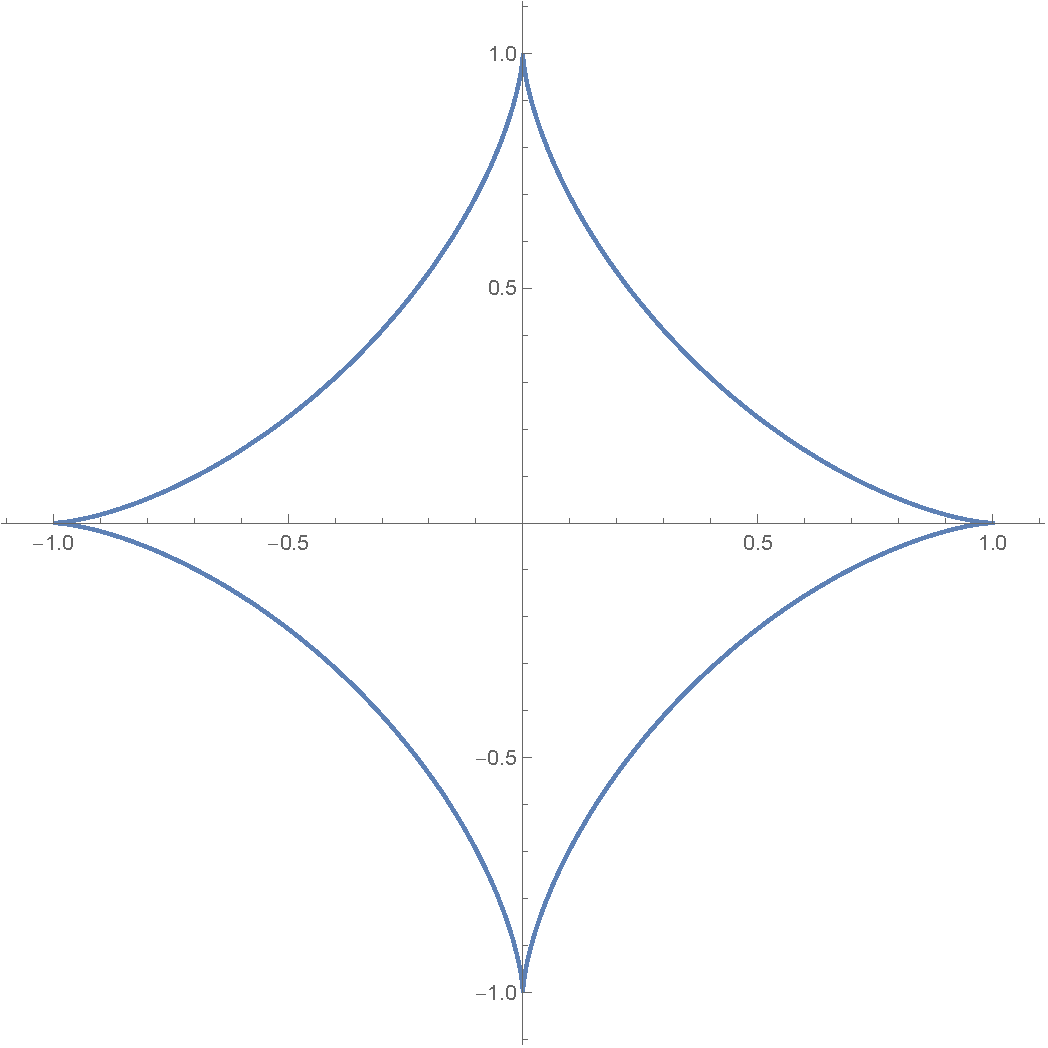
\includegraphics[height=4.5cm, width=4.5cm]{1.pdf}

\end{center}

(2)球冠面积:$A=2\pi Rh.$

(3)高次方正弦余弦和,再增幂,无规律

\centerline{$\sin^4x+\cos^4x=1-2\sin^2x\cos^2x,
\qquad
\sin^6x+\cos^6x=1-3\sin^2x\cos^2x.$}

\newpage

\section{无穷级数}

\subsection{数项级数}

\no1.基础知识

\no(1)无穷级数:$\dis\sumn u_n$, 部分和:$S_n=\sumkn u_k$, 
级数收敛:$\limn S_n=S$, 称$S$为级数的和.

\no$\ \ \ \ $余和:$r_n=S-S_n=\dis\sum\limits_{k=n+1}^\infty u_k$, 
级数收敛$\Longleftrightarrow\limn r_n=0.$

\no(2)性质

\begin{enumerate}[itemindent=1.4em, label=(\alph*)]

\item $k\neq0,\ \sumn ku_n$与$\sumn u_n$的敛散性相同

\item $\sumn u_n,\ \sumn v_n$收敛$\Longrightarrow\sumn(u_n\pm v_n)$
收敛, 

\vspace{0.2cm}

$\quad$收敛$\pm$收敛$=$收敛, 收敛$\pm$发散$=$发散, 发散$\pm$发散$=$不一定 

\item 有限项的变化不影响级数的敛散性

\item 收敛级数任意\textcolor[rgb]{1,0,0}{加括号},仍收敛;
发散级数任意\textcolor[rgb]{1,0,0}{去括号(拆项)},仍发散

\item 级数收敛的必要条件:$\limn u_n=0.$

\end{enumerate}

\no(3)正项级数敛散性判别法

正项级数:$\sumn u_n,\ u_n \textcolor[rgb]{1,0,0}{\gs}0$, 注意$u_n$可以为零, 
正项级数收敛$\Longleftrightarrow$部分和序列有上界

比较判别法:$\forall n\in\mathbb{N},\ 0\ls u_n\ls v_n,\ $
则$\sumn v_n$收敛$\Longrightarrow\sumn u_n$收敛, 
$\sumn u_n$发散$\Longrightarrow\sumn v_n$发散

\vspace{0.3cm}

比较判别法的极限形式:$v_n\neq0,\ \limn \dfrac{u_n}{v_n}=C\longrightarrow$
$\left\{\begin{array}{ll}
0<C<+\infty, &\text{敛散性一致;}\\
C=0,&\sumn v_n\text{收敛}\Longrightarrow\sumn u_n\text{收敛;}\\
C=+\infty,&\sumn u_n\text{发散}\Longrightarrow\sumn v_n\text{发散}.\\
\end{array}\right.$

\vspace{0.3cm}

比值根值法:$\limn\dfrac{u_{n+1}}{u_n}=\rho,\ $或$\limn \sqrt[^n\!]{u_n}=\rho,\ 
\rho<0$收敛; $\rho>1$发散且$\limn u_n\neq0;\ \rho=0$不定.

\vspace{0.2cm}

积分判别法:$f(x)\in C[a,+\infty),f(x)\gs0,\searrow\ ,\ u_n=f(n)\Longrightarrow
\sumn u_n$与$\intd_a^{+\infty} f(x)\dif x$敛散性相同.

\no(4)三个重要级数

等比级数:$\sumn ar^{n-1}\longrightarrow\left\{\begin{array}{l}
|r|<1\text{时收敛},\ S=\dfrac{a}{1-r}\\
|r|\gs1\text{时发散}\\
\end{array}\right.$

P-级数:$\sumn \dfrac{1}{n^p},\ p\ls1$发散, $p>1$收敛

\vspace{0.3cm}

P-对数级数:$\dis\sum\limits_{n=2}^{\infty}\dfrac{1}{n\ln^pn},\ p\ls1$发散, $p>1$收敛

\vspace{0.3cm}

\no(5)任意项级数,绝对收敛

绝对收敛:$\sumn|u_n|$收敛; $\qquad$条件收敛:$\sumn|u_n|$发散, $\sumn u_n$收敛

\vspace{0.2cm}

绝对收敛$\Longleftrightarrow$正项负项级数都收敛;
$\qquad$
条件收敛$\Longleftrightarrow$正项负项级数均发散

交错级数:$u_n>0,\ \sumn(-1)^{n-1}u_n$, 

Leibniz判别法(充分条件):
$\limn u_n=0,\ u_n\gs u_{n+1}$则收敛,且$S\ls u_1,\ |r_n|\ls u_{n+1}.$

\vspace{0.3cm}

\no2. \textcolor[rgb]{1,0,0}{裂项相消法}:$u_n=x_n-x_{n-1},\ \sumn u_n=x_1-\limn x_{n+1}
\Longrightarrow\left\{\limn a_n\text{存在}\Longleftrightarrow\sumn(a_n-a_{n-1})
\text{收敛}\right\}$

\vspace{0.3cm}

\textbf{例1}:$u_{n+1}=u_n^2-u_n+1\Longrightarrow\dfrac{1}{u_n}
=\dfrac{1}{u_n-1}-\dfrac{1}{u_{n+1}-1}.$

\textbf{例2}:$\arccot\big[1+n(n+1)\big]=\arccot n-\arccot (n+1).$

\no3. 一道不太好想的证明题:$p\gs1,\ \sumn\dfrac{1}{(n+1)\sqrt[^p\!]{n}}<p.$

\textbf{证}:由Lagrange中值定理可知

$\dis\frac{1}{n}-\frac{1}{n+1}
=\Bigg(\dfrac{1}{\sqrt[^p\!]{n}}\Bigg)^p-\Bigg(\dfrac{1}{\sqrt[^p\!]{n+1}}\Bigg)^p
=p\cdot\xi_n^{p-1}\Bigg(\dfrac{1}{\sqrt[^p\!]{n}}-\dfrac{1}{\sqrt[^p\!]{n+1}}\Bigg),\ 
\dfrac{1}{\sqrt[^p\!]{n+1}}<\xi_n<\dfrac{1}{\sqrt[^p\!]{n}}.$

\vspace{0.3cm}

原式:$\dfrac{1}{(n+1)\sqrt[^p\!]{n}}=\dfrac{n^{1-\tfrac{1}{p}}}{n(n+1)}
=n^{\tfrac{p-1}{p}}\left(\dfrac{1}{n}-\dfrac{1}{n+1}\right)
=p\cdot n^{\tfrac{p-1}{p}}\cdot\xi_n^{p-1}\Bigg(\dfrac{1}{\sqrt[^p\!]{n}}-\dfrac{1}{\sqrt[^p\!]{n+1}}\Bigg)$,

\vspace{0.3cm}

其中, $n^{\tfrac{p-1}{p}}\cdot\xi_n^{p-1}=\Big(\sqrt[^p\!]{n}\cdot\xi_n\Big)^{p-1}<
\Bigg(\sqrt[^p\!]{n}\cdot\dfrac{1}{\sqrt[^p\!]{n}}\Bigg)^{p-1}=1
\Longrightarrow\dfrac{1}{(n+1)\sqrt[^p\!]{n}}<p\cdot
\Bigg(\dfrac{1}{\sqrt[^p\!]{n}}-\dfrac{1}{\sqrt[^p\!]{n+1}}\Bigg),$

\vspace{0.3cm}

$\Longrightarrow\sumn\dfrac{1}{(n+1)\sqrt[^p\!]{n}}
<\sumn p\cdot\Bigg(\dfrac{1}{\sqrt[^p\!]{n}}-\dfrac{1}{\sqrt[^p\!]{n+1}}\Bigg)=p.$
\qed

\vspace{0.3cm}

\no4.子数列:根本原则$\longrightarrow$ \textcolor[rgb]{1,0,0}{单调必放缩}

$\{a_n\}\gs0\searrow\ ,\sumn a_n$收敛$\Longrightarrow\limn na_n=0.$

\textbf{证}:$S_{2n}-S_n\gs na_{2n}\longrightarrow0\Longrightarrow 2na_{2n}
\longrightarrow0,\ (2n+1)a_{2n+1}\ls(2n+1)a_{2n}\longrightarrow0.$
\qed

\no5.递推数列:求和则用比值法

\textbf{例}:Fibonacci数列,$F_1=1,\ F_2=1,\ F_n=F_{n-1}+F_{n-2},\ n\gs3.$则

(1) $\dfrac{3}{2}F_{n-1}\ls F_n\ls2F_{n-1}\Longrightarrow
\left(\dfrac{3}{2}\right)^{n-1}<F_n<2^{n+1}.$

\vspace{0.2cm}

(2) $\limn\dfrac{F_n}{F_{n+1}}=\dfrac{\sqrt{5}+1}{2}=0.618.$

\vspace{0.2cm}

(3) $F_n=\dfrac{1}{\sqrt{5}}\Bigg[\left(\dfrac{\sqrt{5}+1}{2}\right)^n-\left(\dfrac{1-\sqrt{5}}{2}\right)^n\Bigg].$

\vspace{0.2cm}

(4) $\Big|F_{n+1}^2-F_{n+2}F_n\Big|=1.$

\no6.余项处理技巧:数列与数列和的关系, 
$\{u_n\}\gs0\Longrightarrow S_n\nearrow\ \Longrightarrow S_n$可放缩

\textbf{例}:$\sumn u_n>0$发散$,\ \limn u_n=+\infty
\Longrightarrow\sumn \dfrac{u_n}{S_n}$发散.

\vspace{0.2cm}

\textbf{证}:余项$\dis r_n=\sum\limits_{k=n+1}^\infty\dfrac{u_k}{S_k}\gs
\sum\limits_{k=n+1}^{n+p}\dfrac{u_k}{S_k}\gs
\dfrac{1}{S_{n+p}}\sum\limits_{k=n+1}^{n+p}u_k
=\dfrac{S_{n+p}-S_n}{S_{n+p}}=1-\dfrac{S_n}{S_{n+p}},\ 
p$充分大时,

\vspace{0.2cm}

$\dis\dfrac{S_n}{S_{n+p}}<\frac{1}{2}\ \Big(\text{此时}n\text{固定而}p\text{趋于无穷}\Big)
\Longrightarrow
r_n\gs1-\dfrac{S_n}{S_{n+p}}\gs\frac{1}{2}\nrightarrow0
\Longrightarrow\sumn \dfrac{u_n}{S_n}$发散.

\vspace{0.2cm}

余项者, 先固定一个$n,\ $取$n+p,\ p$动而$n$不动. 若$\limn u_n=+\infty$
则$\dis\dfrac{S_n}{S_{n+p}}<\frac{1}{2}.$\qed

\vspace{0.2cm}

\no7.存在极限$\limn a_n=a\Longrightarrow n$充分大时,$\ 0<\dfrac{|a|}{2}<|a|<2|a|,\ $
后可放缩. 对于$a>0,\ a>1,\ a<1,\ $可取$a>b>0,\ a>b>1,\ a<b<1,\ $得中间值$b$, 由不等关系构造不等式.

\vspace{0.2cm}

\no8. $\dis\sum\limits_{n=2}^\infty\ln\Bigg(1+\dfrac{(-1)^n}{n^p}\Bigg),\ p>0
\Longrightarrow p>1$绝对收敛,$\ \dfrac{1}{2}<p\ls1$条件收敛,$\ 0<p\ls\dfrac{1}{2}$发散.

\vspace{0.2cm}

\no9. 根号下不展开,分子有理化消根号

\no10. 两个特殊的级数

(1)$\ u_n\to0$ but diverges: 
$\dis\sum\limits_{n=2}^\infty\dfrac{(-1)^n}{\sqrt{n}+(-1)^n}.$

(2) 收敛的正项级数$n\to0,\ a_n\neq o\left(\dfrac{1}{n}\right):\ k\in\mathbb{N}^*,\ 
a_n=\left\{\begin{array}{ll}
\dfrac{1}{n},&n=k^2\\
\dfrac{1}{n^2},&n\neq k^2\\
\end{array}\right.$, 极限不存在

\no11. \textcolor[rgb]{1,0,0}{Cauchy–Schwarz inequality}

The Cauchy–Schwarz inequality states that for all vectors $\stackrel{\rightarrow}{u}$ and $\stackrel{\rightarrow}{v}$ of an inner product space it is true that

\centerline{\textcolor[rgb]{0,0,1}{$\displaystyle \left|\left< \stackrel{\rightarrow}{u} ,\stackrel{\rightarrow}{v} \right> \right|^{2}\ls \left< \stackrel{\rightarrow}{u} ,\stackrel{\rightarrow}{u} \right> \cdot \left< \stackrel{\rightarrow}{v} ,\stackrel{\rightarrow}{v} \right> ,$}}

where $\displaystyle \langle \cdot ,\cdot \rangle $ is the inner product. 

\textcolor[rgb]{1,0,0}{$\mathbb{R}^2$ (ordinary two-dimensional space)}

In the usual 2-dimensional space with the dot product, let $\displaystyle \stackrel{\rightarrow}{v}=(v_{1},v_{2})$ and ${\displaystyle \stackrel{\rightarrow}{u}=(u_{1},u_{2})}$. The Cauchy–Schwarz inequality is that

\centerline{\textcolor[rgb]{0,0,1}{${\displaystyle \left< \stackrel{\rightarrow}{u},\stackrel{\rightarrow}{v}\right>^{2}=\Big(\left\|\stackrel{\rightarrow}{u}\right\|\left\|\stackrel{\rightarrow}{v}\right\|\cos \theta \Big)^{2}\ls \left\|\stackrel{\rightarrow}{u}\right\|^{2}\left\|\stackrel{\rightarrow}{v}\right\|^{2}} ,$}}

where $\theta$  is the angle between $\stackrel{\rightarrow}{u}$ and $\stackrel{\rightarrow}{v}$.

The form above is perhaps the easiest in which to understand the inequality, since the square of the cosine can be at most 1, which occurs when the vectors are in the same or opposite directions. It can also be restated in terms of the vector coordinates ${\displaystyle v_{1},\ v_{2},\ u_{1}}$ and $u_{2}$ as

\centerline{\textcolor[rgb]{0,0,1}{${\displaystyle (u_{1}v_{1}+u_{2}v_{2})^{2}\ls \big(u_{1}^{2}+u_{2}^{2}\big)\cdot \big(v_{1}^{2}+v_{2}^{2}\big)},\ $}}

where equality holds if and only if the vector $(u_{1},u_{2})$ is in the same or opposite direction as the vector ${\displaystyle (v_{1},v_{2})}$, or if one of them is the zero vector.

\textcolor[rgb]{1,0,0}{$\mathbb{R}^n$ (n-dimensional Euclidean space)}

In Euclidean space ${\displaystyle \mathbb {R} ^{n}}$ with the standard inner product, the Cauchy–Schwarz inequality is

\centerline{\textcolor[rgb]{0,0,1}{${\displaystyle \left(\sum _{i=1}^{n}u_{i}v_{i}\right)^{2}\ls \left(\sum _{i=1}^{n}u_{i}^{2}\right)\left(\sum _{i=1}^{n}v_{i}^{2}\right)} .$}}

The Cauchy–Schwarz inequality can be proved using only ideas from elementary algebra in this case. Consider the following quadratic polynomial in $x$

\centerline{\textcolor[rgb]{0,0,1}{${\displaystyle 0\ls (u_{1}x+v_{1})^{2}+\cdots +(u_{n}x+v_{n})^{2}=\left(\sumin u_{i}^{2}\right)x^{2}+2\left(\sumin u_{i}v_{i}\right)x+\sumin v_{i}^{2}.} $}}

Since it is nonnegative, it has at most one real root for $x$, hence its discriminant is less than or equal to zero. That is,

\centerline{\textcolor[rgb]{0,0,1}{${\displaystyle \left(\sumin u_{i}v_{i}\right)^{2}-\sumin {u_{i}^{2}}\cdot \sumin {v_{i}^{2}}\ls 0,} $}}

which yields the Cauchy–Schwarz inequality.

\textcolor[rgb]{1,0,0}{$L^2$ (square-integrable space)}

For the inner product space of square-integrable complex-valued functions, one has

\centerline{\textcolor[rgb]{0,0,1}{${\displaystyle \left|\int _{\mathbb {R} ^{n}}f(x){\overline {g(x)}}\,\dif x\right|^{2}\ls \int _{\mathbb {R} ^{n}}|f(x)|^{2}\,\dif x\cdot \int _{\mathbb {R} ^{n}}|g(x)|^{2}\,\dif x.} $}}

\vspace{0.3cm}

\textbf{例}:$\sumn a_n^2$ converges $\Longrightarrow\sumn \dfrac{a_n}{n}\ls\sumn \left|\dfrac{a_n}{n}\right|\ls\sqrt{\sumn a_n^2}\cdot\sqrt{\sumn \dfrac{1}{n^2}}$ converges.

\no12. 数列放缩

$a_n\searrow\ ,\ a_n+a_{n+2}=\dfrac{1}{n+1}\Longrightarrow
\dfrac{1}{2(n+1)}\ls a_n\ls\dfrac{1}{n+1}.$

\no13.正项级数收敛$\Longrightarrow$幂次大于此正项级数的级数亦收敛

\textbf{例}:$\sumn a_n$ converges$\Longrightarrow$ when $n$ is large enough, 
$|a_n|\ls1\Longrightarrow|a_n|^p\ls|a_n|\Longrightarrow\sumn a_n^p$ converges.

\vspace{0.2cm}

\no14.正弦级数:二项展开, 配凑$\pi$的系数为偶数

\textbf{例}:$\sumn \sin\pi\Big(3+\sqrt{5}\Big)^n+\sumn \sin\pi\Big(3-\sqrt{5}\Big)^n
=0,\ \sumn \sin\pi\Big(3-\sqrt{5}\Big)^n\ls\sumn \pi\Big(3-\sqrt{5}\Big)^n,\ 3-\sqrt{5}<1\Longrightarrow\sumn \pi\Big(3-\sqrt{5}\Big)^n$ converges $\Longrightarrow\sumn \sin\pi\Big(3-\sqrt{5}\Big)^n$ converges $\Longrightarrow\sumn \sin\pi\Big(3+\sqrt{5}\Big)^n$ converges.

\vspace{0.2cm}

\no15.一些解题技巧

级数相除,配系数凑零值级数展开;双重无穷定积分,变量耦合化一积;

无穷乘积取幂指,则化为无穷级数

\no16.证明同敛散($\sim$)可夹逼

\textbf{例}:$f(x)\in C[a,+\infty),\ f(x)\gs0,\ a=a_0<a_1<a_2<\cdots<a_n<\cdots,\ 
\limn a_n=+\infty,$

$\ u_n=\intd_{a_{n-1}}^{a_n}f(x)\dif x,\ \intd_0^\infty f(x)\dif x\sim\sumn u_n,$ 
and if converge, $\intd_0^\infty f(x)\dif x=\sumn u_n.$

\vspace{0.2cm}

\no17. \textcolor[rgb]{1,0,0}{压缩映射}原理:级数收敛$\Longleftrightarrow$数列收敛

(1) $f(x)\in C(-\infty,+\infty),\ \exists\ 0<\alpha<1,\ \forall\ x,y,\ |f(x)-f(y)|\ls\alpha|x-y|,\ 
\exists$ one $x_0\ s.t.\ x_0=f(x_0).$

(2) $f(x)\in C^1(-\infty,+\infty),\ |f'(x)|\ls\alpha<1,$ let $x_1\in(-\infty,+\infty),\ 
x_{n+1}=f(x_n)\Longrightarrow\exists\limn x_n=x_0.$

\subsection{函数项级数}

\no1.基础知识

\no(1) 函数项级数:$\sumn u_n(x)=u_1(x)+u_2(x)+\cdots+u_n(x)+\cdots,\ $

\vspace{0.2cm}

收敛域:所有收敛点构成的集合;

和函数:$S(x)=$

\no(2)幂级数:$\sumnz a_nx^n$

\vspace{0.2cm}

Abel引理:收敛圆盘,边界不定;

收敛半径:$R=\textcolor[rgb]{1,0,0}{\dis\dfrac{1}{\varlimsup\limits_{n\to\infty}\sqrt[^n\!]{|a_n|}}}
=\limn\left|\dfrac{a_n}{a_{n+1}}\right|
=\limn\dfrac{1}{\sqrt[^n\!]{|a_n|}}$

\vspace{0.2cm}

收敛区间:$(-R,R)$

收敛域:单独计算$|x|=R$两个数项级数得出收敛域

换元法:$t=x+x_0,\ t=x^2,\cdots$

和函数:$S(x)=\sumnz a_nx^n$,在收敛域上连续;逐项可积;逐项可导

\vspace{0.2cm}

乘法运算:$\left(\sumnz a_nx^n\right)\left(\sumnz b_nx^n\right)
=\sumnz(a_nb_0+a_{n-1}b_1+\cdots+a_0b_n)x^n
=\sumnz\left(\sumizn a_{n-i}b_i\right)x^n.$

\vspace{0.2cm}

\no(3) 幂级数展开

Taylor series: $f(x)=\sumnz\dfrac{f^{(n)}(x_0)}{n!}(x-x_0)^n,\ x\in$收敛域, 
收敛到$f(x)\Longleftrightarrow\limn R_n(x)=0.$

\vspace{0.2cm}

Maclaurin series: $f(x)=\sumnz\dfrac{f^{(n)}(x_0)}{n!}x^n.$

\vspace{0.2cm}

\no(4)一些特殊函数的幂级数展开

\vspace{0.2cm}

$\sin x=\sumnz(-1)^n\dfrac{x^{2n+1}}{(2n+1)!},\ x\in(-\infty,+\infty),\qquad
\cos x=\sumnz (-1)^n\dfrac{x^{2n}}{(2n)!},\ x\in(-\infty,+\infty),$

\vspace{0.2cm}

$e^x=\sumnz\dfrac{x^n}{n!},\ x\in(-\infty,+\infty),\qquad\qquad(1+x)^\alpha=\sumnz\binom{\alpha}{n}x^n,\ x\in(-1,1),\ |x|=1$不定,

\vspace{0.2cm}

$\dfrac{1}{1+x}=\sumnz(-1)^nx^n,\ x\in(-1,1),\qquad
\dfrac{1}{1-x}=\sumnz x^n,\ x\in(-1,1),$

\vspace{0.2cm}

$\ln(1+x)=\sumn\dfrac{ (-1)^{n-1}x^{n}}{n},\ 
x\in(-1,1],\qquad
\ln(1-x)=-\sumn\dfrac{x^{n}}{n},\ x\in[-1,1),$

\vspace{0.2cm}

$\dfrac{1}{2}\ln\dfrac{1+x}{1-x}=\sumn\dfrac{x^{2n-1}}{2n-1},\ x\in(-1,1),
\qquad\quad
\arctan x=\sumnz(-1)^n\dfrac{x^{2n+1}}{2n+1},\ x\in[-1,1].$

\vspace{0.2cm}

\textbf{注}:这些收敛域中, 在$|x|=1$处是否闭合一般看是否能形成交错级数.

\no(5) Fourier series

(a) $f(x)\sim\dfrac{a_0}{2}+\sumn(a_n\cos nx+b_n\sin nx),\ $where

\vspace{0.2cm}

$\quad a_0=\dfrac{1}{\pi}\intd_{-\pi}^{\pi}f(x)\dif x,\ 
a_n=\dfrac{1}{\pi}\intd_{-\pi}^{\pi}f(x)\cos nx\dif x,\ 
b_n=\dfrac{1}{\pi}\intd_{-\pi}^{\pi}f(x)\sin nx\dif x,\ n\in\mathbb{N}^*.$

(b)收敛的充分条件

\textcolor[rgb]{1,0,0}{Dirichlet conditions:}

 (i)   $f$ must be absolutely integrable over a period.

(ii)  $f$ must be of bounded variation in any given bounded interval.

(iii) $f$ must have a finite number of discontinuities in any given bounded interval, and the discontinuities cannot be infinite.

\textcolor[rgb]{1,0,0}{Dirichlet's theorem:}

Assuming $f$ is a periodic function of period $2\pi$ with Fourier series expansion where

\centerline{\textcolor[rgb]{0,0,1}{${\displaystyle a_{n}={\frac {1}{2\pi }}\int _{-\pi }^{\pi }f(x)e^{-inx}\,\dif x.} $}}

The analogous statement holds irrespective of what the period of f is, or which version of the Fourier expansion is chosen. 

If $f$ satisfies Dirichlet conditions, then for all $x$, we have that the series obtained by plugging $x$ into the Fourier series is convergent, and is given by

\centerline{\textcolor[rgb]{0,0,1}{${\displaystyle \sum _{n=-\infty }^{\infty }a_{n}e^{inx}={\frac {1}{2}}\big(f(x+)+f(x-)\big)}.$}}

\no(6) Fourier sine series: $f(x)$ is an odd function,

$a_n=0,\ n\in\mathbb{N},\ b_n=\dfrac{2}{\pi}\intd_0^\pi f(x)\sin nx\dif x,\ 
f(x)\sim\sumn b_n\sin nx.$

\no(7) Fourier cosine series: $f(x)$ is an even function,

$a_0=\dfrac{2}{\pi}\intd_0^\pi f(x)\dif x,\ a_n=\dfrac{2}{\pi}\intd_0^\pi f(x)\cos nx\dif x,\ 
b_n=0,\ n\in\mathbb{N}^*,\ f(x)\sim\dfrac{a_0}{2}+\sumn a_n\cos nx.$

\no(8)以$2l$为周期的函数展开为Fourier series

$f(x)\sim\dfrac{a_0}{2}+\sumn\left(a_n\cos\dfrac{n\pi x}{l}+b_n\sin\dfrac{n\pi x}{l}\right),$

$ a_0=\dfrac{1}{l}\intd_{-l}^lf(x)\dif x,\ a_n=\dfrac{1}{l}\intd_{-l}^lf(x)\cos\dfrac{n\pi x}{l}\dif x,\ b_n=\dfrac{1}{l}\intd_{-l}^lf(x)\sin\dfrac{n\pi x}{l}\dif x,\ n\in\mathbb{N}^*.$

\no(9)一些积分技巧

$\intd x\sin nx\dif x=-\dfrac{x\cos nx}{n}+\dfrac{\sin nx}{n^2},
\qquad
\intd x\cos nx\dif x=\dfrac{x\sin nx}{n}+\dfrac{\cos nx}{n^2},$

\vspace{0.2cm}

$\intd x^2\sin nx\dif x=-\dfrac{x^2\cos nx}{n}+\dfrac{2}{n}\intd x\cos nx\dif x,
\qquad
\intd x^2\cos nx\dif x=-\dfrac{x^2\sin nx}{n}-\dfrac{2}{n}\intd x\sin nx\dif x,$

\vspace{0.2cm}

$x=2\sumn(-1)^{n+1}\dfrac{\sin nx}{n},
\qquad
x^2=\dfrac{1}{3}\pi^2+4\sumn(-1)^n\dfrac{\cos nx}{n^2}$

\no2.幂级数的收敛域

(1) $\sumnz a_nx^n,\ \sumnz b_nx^n$的收敛半径分别为$R_a,\ R_b,$ 收敛域$I_a\neq I_b,$

\centerline{$\sumnz (a_n\pm b_n)x^n,\ R_a\neq R_b\Longrightarrow I=I_a\cap I_b.$}

\vspace{0.2cm}

(2)求导或积分,收敛半径不变

(3)公式法:
$R=\textcolor[rgb]{1,0,0}{\dis\dfrac{1}{\varlimsup\limits_{n\to\infty}\sqrt[^n\!]{|a_n|}}}
=\limn\left|\dfrac{a_n}{a_{n+1}}\right|
=\limn\dfrac{1}{\sqrt[^n\!]{|a_n|}}$

\vspace{0.2cm}

(4)若缺项,则换元:$t=x^2,\cdots$

\no3.幂级数展开

\begin{enumerate}[itemindent=1.4em, label=(\arabic*)]

\item 裂项变形,换元,利用已知展开式,加减乘复合

\item 逐项积分或逐项微分

\item 待定系数法,一般是分式,假设展开,比较系数

\item 定义法,Taylor series

\item $\cos x,\ \sin x$遇到$e^x$可考虑Euler公式:$e^{ix}=\cos x+i\sin x$

\item 直接展开,微分方程求$n$阶导数找递推公式

\textbf{例}:$y=\dfrac{\arcsin x}{\sqrt{1-x^2}}\Longrightarrow
y'=\dfrac{1}{1-x^2}+\dfrac{x}{1-x^2}y.$

\end{enumerate}

\no7.幂级数求和

\begin{enumerate}[itemindent=1.4em, label=(\arabic*)]

\item 配凑$x^n$利用展开

\item 先积分再求导:$\left\{\begin{array}{l}
\text{先导再积}+C\\
\text{先积再导不}+C\\
\end{array}\right.$

\item 方程式法:$\left\{\begin{array}{l}
\text{求导,和函数复现}\\
\text{递推数列,列}S(x)\text{的方程}\\
\end{array}\right.$

\end{enumerate}

\no8.一般函数项级数

\begin{enumerate}[itemindent=1.4em, label=(\arabic*)]

\item 函数项级数换元化为幂级数;若为正向级数亦可直接做

\item 双重求和换序:与该求和变量无关的量可以提出去

\textbf{例}:$\sumnz \dfrac{1}{n!}\sumkz\dfrac{k^nx^k}{k!}=
\sumkz\dfrac{x^k}{k!}\sumnz\dfrac{k^n}{n!}$

\end{enumerate}

\newpage

\section{微分方程}

\subsection{初等积分法与线性方程}

\subsection{微分方程的应用}

\end{spacing}

\end{document}